% ==========================================================================
% ======================== Dokumentace k PC 1.0 ;-) ========================
% ==========================================================================

% Ověřeno, prošlo bez jediné připomínky - při dodržení následujících pokynů:
% - SPRÁVNĚ vyplnit titulní stranu (!!!)
% - Nadpisy používat v pořadí (zanoření):
% 		- chapter (celá kapitola)
%		- section
% 		- subsection, subsubsection ... 
% - Pro pomlčky V TEXTU používat -- (doslova 2 mínusy). Neplatí pro rozsahy
%	(0-9), spojovníky typu xxx-li apod.
% - Uvozovky - používat české \uv{hezké uvozovky}.
% - Zvýrazňovat \textit{kurzívou}.
% - Názvy modulů, funkcí psát \texttt{neproporcionálním fontem}.
% - URL psát do \url{}
% - In-line matematické výrazy přímo do řádky $uzavřené do dolarů$, složitější
%	na samostatnou řádku $$do dvojitých$$.
% - Pokud např. v zadání zmiňujete LATEX a TEX, použít \latex resp. \tex.

% - Pozor na předložky a spojky - nesmí se vyskytovat na konci řádku => použít
%	nedělitelnou mezeru (~).
% - Nové odstavce dvojitým odřádkováním.

% OBRÁZKY	- Vektorově (!!!) - Illustrator, free Inkscape.
% 			- Rastrově vkládat jen screeny obrazovky.
%			- V textu pak odkazovat pomocí \ref{img1}.
%			- Pro úpravu velikosti změnit scale.
% 	\begin{figure}[h]
%		\centering
%		\includegraphics[scale=1.0]{soubor.pdf/png}
%		\caption{Popisek}
%		\label{img1}
%	\end{figure}

% PŘELOŽENÍ
% - Nainstalovat doporučený MiKTeX.
% - "pdflatex <nazev-souboru>.tex"
% - Pro správné vygenerování odkazů, obsahu nutné vždy spustit 2x (!!!)
% - Pro zjednodušení stačí spouštět přibalený bat, který to udělá sám ;)

% ^^^^^^^^^^^^^^^^^^^^^^^^^^^^^^^^^^^^^^^^^^^^^^^^^^^^^^^^^^^^^^^^^^^^^^^^^^
% ^^^^^^^^^^^^^^^^^ !!!!!!!!!SMAZAT PŘI ODEVZDÁNÍ!!!!!!!!! ^^^^^^^^^^^^^^^^^
% ^^^^^^^^^^^^^^^^^^^^^^^^^^^^^^^^^^^^^^^^^^^^^^^^^^^^^^^^^^^^^^^^^^^^^^^^^^

\documentclass[
12pt,
a4paper,
pdftex,
czech,
titlepage
]{report}

\usepackage[czech]{babel}
\usepackage[utf8]{inputenc}
\usepackage{lmodern}
\usepackage{textcomp}
\usepackage[T1]{fontenc}
\usepackage{amsfonts}
\usepackage{titlesec}
\usepackage{graphicx}
\usepackage{framed}
\usepackage{amsmath}

\titleformat{\chapter}
  {\normalfont\LARGE\bfseries}{\thechapter}{1em}{}
\titlespacing*{\chapter}{0pt}{0ex plus 1ex minus .2ex}{2.0ex plus .2ex}
\setlength\parindent{0pt}

\begin{document}

\begin{titlepage}
	\vspace*{-2cm}
	{\centering
\includegraphics[scale=1.0]{logo.pdf}\par}
	\centering
	\vspace*{2cm}
	{\Large Semestrální práce z KIV/PC\par}
	\vspace{1.5cm}
	{\Huge\bfseries Vyhledávání cest v grafu technikou DFS\par}
	\vspace{2cm}

	{\Large Petr Hlaváč\par}
	{\Large A15B0037P\par}
	{\Large petrh@students.zcu.cz\par}

	\vfill

	{\Large 1.\,12.\,2017}
\end{titlepage}

\tableofcontents
\thispagestyle{empty}
\clearpage

\chapter{Zadání}
Naprogramujte v ANSI C přenositelnou \textbf{konzolovou aplikaci}, která bude \textbf{procházet graf technikou DFS} (Depth--First--Search). Vstupem aplikace bude soubor s popisem grafu. Výstupem je pak odpovídající výčet všech cest mezi požadovanými uzly.\\

Program se bude spouštět příkazem \textbf{dfs.exe} <soubor-grafu> <id1> <id2> <maxD>
\begin{itemize}
\item Symbol <soubor-grafu> zastupuje parametr - název vstupního souboru se strukturou grafu.
\item Následují identifikátory (dále jen id) dvou uzlů v grafu <id1> a <id2>, mezi kterými bude spouštěn proces hledání cest.
\item <maxD> je parametr popisující maximální délku cest, které mají být nalezeny.
\end{itemize}

Vámi vyvinutý program tedy bude vykonávat následující činnosti.
\begin{enumerate}
\item Při spuštění bez potřebných parametrů vypíše nápovědu pro jeho správné spuštění a ukončí se.
\item Při spouštění s parametry načtě zadaný vstupní soubor do vhodné struktury reprezentující graf a mezi zadanými uzly najde všechny cesty, jejichž délka nepřekročí konstatnu nastavenou vstupním parametrem.
\end{enumerate}

Váš program může být během testování spuštěn například takto:\\

\framebox[1.1\width]{dfs.exe graph.csv 1 2 4}\\

Při tomto spuštění program vyhledá všechny cesty délky 1 až 4 mezi uzly 1 a 2.\\

Hotovou práci odevzdejte v jediném archivu typu ZIP prostřednictvím automatického odevzdávacího a validačního systému. Postupujte podle instrukcí uvedených na webu předmětu. Archiv nechť obsahuje všechny zdrojové soubory potřebné k přeložení programu, \textbf{makefile} pro Windows i Linux a dokumentaci ve formátu PDF vytvořenou v typografickém systému \TeX, resp. \LaTeX.

\section{Popis činnosti programu}
Program načte vstup ve formátu CSV, který vhodným zbůsobem uloží do paměti pro pozdější prohledávání. Následně spustí algoritmus, jehož výstupem bude seznam všech cest mezi dvěma uzly, které bude vypisovat na standardní výstup ve formátu popsaném dále.

\subsection{Specifikace výstupu programu}
Program bude na standardní výstup vypisovat jednotlivé cesty. Vždy na jeden řádek právě jednu cestu. Cesty budou popsány posloupností id jenotlivých uzlů oddělených pomlčkou (tj. znakem minus,  \uv{\textbf{-}}). následovat bude středník a popisky jednotlicých hran v grafu oddělené čárkou. Za posledním středníkem bude uvedena hodnota sekundární metriky - relevance cesty, podle které budou cesty seřazeny (viz Řazení výstupu).\\

Například tedy pro hledání cest mezi uzly A a B:\\

\textbf{A-B};$h_{1}$;$m_{1}$\\
\textbf{A-F-B};$h_{2}$,$h_{3}$;$m_{2,3}$\\
\textbf{A-W-B};$h_{4}$,$h_{5}$;$m_{4,5}$\\
\textbf{A-F-O-B};$h_{2}$,$h_{6}$,$h_{7}$;$m_{2,6,7}$\\


Kde A, B, F, W, F, ... jsou popisky uzlů grafu, $h_{n}$ jsou ohodnocení hran a $m_{c1,c2...cn}$ je hodnota metrika relevance nalezené cesty.

\subsection{Řazení výstupu}
Cesty budou na standardním výstupu seřazeny podle jejich délky. Pokud bude nalezeno více cest stejné dálky, budou seřezeny podle jejich relevance následujícím způsobem. Popisky grafu nesou informaci o kalendářním datu ve formátu YYYY--MM--DD. Každá cesta budde tedy ohodnocena celým číslem, které bude odpovídat rozdílu v počtu dní mezi nejstarším a nejnovějším datem, následně budou podle toho čísla cesty se shodnou délkou seřazeny vzestupně.\\

Pokud tedy nalezete cestu, kterou budou tvořit tyto 4 hrany s hodnotami:\\

2000--01--15,\\
2000--01--04,\\
2000--01--19,\\
2000--01--24,\\

vypočte se hodnota metriky jako počet dnů mezi daty 2000--01--04 a 2000--01--24, což je 20.

\section{Podrobné zadání}
Originální nezkrácené zadání je možné nalézt na adrese:\\

http://www.kiv.zcu.cz/studies/predmety/pc/doc/work/sw2017-02.pdf

\setcounter{page}{1}

\chapter{Analýza úlohy}
Úloha se skládá z následujícíh kroků:
\begin{enumerate}
	\item Načtení vstupních dat.
	\item Vybrání vhodné datové struktury.
	\item Modifikace algoritmu DFS pro hledání všech cest mezi dvěma body.
\end{enumerate}

\section{Načtení vstupních dat}
CSV nebo-li Comma-separeted-values je jednoduchý souborový formát určený pro výměnu tabulkových dat.\\

Ukázka vstupního souboru ve formátu CSV
\begin{framed}
	1;2;2007--02--16\\
	1;2;2008--02--15\\
	1;3;2007--10--26\\
	1;4;2007--10--30\\
	3;2;2007--10--11\\
	3;6;2007--06--14\\
	3;7;2007--08--14\\
	3;9;2008--03--05\\
	4;2;2007--10--05\\
	5;1;2007--02--04
\end{framed}

Data jsou formátovány ve stylu idUzlu1; idUzlu2; hodnotaHrany\\

Jedna řádka vstupního souboru představuje jednu hranu. Bude tedy vhodné načítat a zpracovávat data po řádcích. Formát CSV nám práci s daty velmi ulehčí, neboť nebude příliš náročné data v řádce rozdělit za pomoci znaku~\uv{\textbf{;}}.

\section{Vybrání vhodné datové struktury}
Pro reprezentaci grafu se využívají následující struktury:
\begin{enumerate}
	\item Matice sousednosti
	\item Spojový seznam
\end{enumerate}

\subsection{Matice sousednoti}
Matice sousednosti má velikost $V \times V$ kde $V$ je počet uzlů. Vzhledem k faktu, že máme ohodnocené hrany grafu vložíme na pozice v matici, kde se nachází hrana její hodnotu a na pozice kde hrana není nějakou specialní hodnotu v našem případě (NULL). Hrany v grafu jsou zadány jako neorientované, tudíž matice bude symetrická viz vzorová matice stavené pro výše zmíněná vstupní data.\\

$\begin{matrix}
 0 & 1 & 2 & 3 & 4 & 5 & 6 & 7 & 8 & 9 \\
 1 & NULL & h1,h2 & h3 & h4 & h10 & NULL & NULL & NULL & NULL \\
 2 & h1,h2 & NULL & h5 & h9 & NULL & NULL & NULL & NULL & NULL \\
 3 & h3 & h5  & NULL & NULL & NULL & h6 & h7 & NULL & h8 \\
 4 & h4 & h9 & NULL & NULL & NULL & NULL & NULL & NULL & NULL \\
 5 & h10 & NULL & NULL & NULL & NULL & NULL & NULL & NULL & NULL \\
 6 & NULL & NULL & h6 & NULL & NULL & NULL & NULL & NULL & NULL \\
 7 & NULL & NULL & h7 & NULL & NULL & NULL & NULL & NULL & NULL \\
 8 & NULL & NULL & NULL & NULL & NULL & NULL & NULL & NULL & NULL \\
 9 & NULL & NULL & h8 & NULL & NULL & NULL & NULL & NULL & NULL \\
\end{matrix}$\\

Neboť je matice pro orientované hrany simetrické, lze ji z paměťových důvodů polovinu zanedbat.
Uložená matice by tedy vypadala takto.\\

$\begin{matrix}
0 & 1 & 2 & 3 & 4 & 5 & 6 & 7 & 8 & 9 \\
1 & NULL  \\
2 & h1,h2 & NULL  \\
3 & h3 & h5  & NULL  \\
4 & h4 & h9 & NULL & NULL  \\
5 & h10 & NULL & NULL & NULL & NULL  \\
6 & NULL & NULL & h6 & NULL & NULL & NULL \\
7 & NULL & NULL & h7 & NULL & NULL & NULL & NULL \\
8 & NULL & NULL & NULL & NULL & NULL & NULL & NULL & NULL  \\
9 & NULL & NULL & h8 & NULL & NULL & NULL & NULL & NULL & NULL \\
\end{matrix}$\\

Pokud se na tuto matici podíváme pozorně zjistíme, že jde v podstatě o reprezentaci Spojovým seznamem. Jedinou výhodou je přístup na dané hrany ve složitosti $O(1)$, neboť matice je reprezentována polem. Tato výhoda má ale ovšem i negativa. Spočívají v tom, že je třeba uložit pole, které je stejně veliké jako id největšího vrcholu v našem grafu. V případě, který nastal i zde, je tedy možné že budeme mít v maticí řádky, které jsou uloženy zcela zbytečně například řádek číslo 8.\\

Další nevýhodou, které si můžeme všimnout je násobnost hran. Abychom v matici uchovali více hran mezi dvěma vrcholy. Musí být hrany v matici reprezentovány spojovým seznamem nebo polem. V případ volby pole by každé přidání nové hrany znamenalo zvětší pole o jedna a přepsání všech hodnot do nového pole, což je v při načítání velkého grafu velmi neefektivní. Vhodnější je tedy spojový seznam.\\

Výsledkem této reprezentace je tedy matice spojových seznamů. Velkou výhodou je přístup k hranám vrcholů v $O(1)$. Nevýhodou může být v některých případech grafů zbytečně velká paměťová složitost a také složitost implementace.


\subsection{Spojový seznam}
Struktura spojového seznamu znamené, že máme pro každý vrchol vytvořen spojový seznam hran, které z něho vycházejí a v kterých je uloženo id souseda a ohodnocení hrany. Spojový seznam pro výše zmíněna data by vypadal takto.\\

\begin{figure}[!h]
	\centering
	 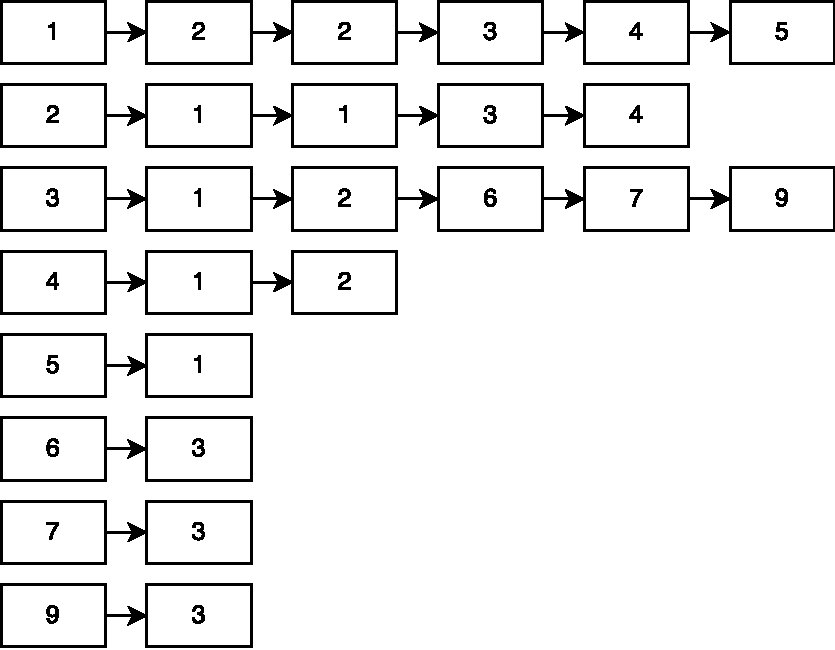
\includegraphics[scale=0.75]{spojak.pdf}
	\caption{Reprezentace grafu spojovým seznamem}
\end{figure}

Neorientované hrany jsou vyřešené přidáním stejné hrany k obou vrcholům. Násobné hrany v této implementaci nedělají žádný problém.\\

Vrcholy grafu je možné mít uložené v poli nebo spojovém seznamu. Výhoda pole je přístup k hraném v $O(1)$. Nevýhodou je pamětová náročnost v případě nevyužítí všech indexů pole. Spojový seznam má přístup k vrcholům v $O(n)$, což může program značně zpomalovat v případě velkého počtu vrcholů v grafu. Vhodná volba tedy záleží hlavně na znalosti vstupních dat.

\subsection{Modifikace algoritmu DFS}
Vyjdeme ze základního algoritmu DFS. Budeme potřebovat zásobník a jeden seznam. Ze zadání víme, že naše prohledávání bude omezeno hloubkou. Dále bylo také řečeno, že se jedná o cestu 


\chapter{Implementace}

\chapter{Uživatelská příručka}

\chapter{Závěr}

\end{document}